% % Preamble
% Declare the document class
\documentclass[12pt]{article}
% Packages to use
\usepackage{amsfonts,amsmath,amssymb,authblk,booktabs,graphicx,lineno,longtable,mathtools,rotating,tabularx,upgreek,booktabs}
\usepackage[authoryear]{natbib}
\usepackage[letterpaper,left=1in,right=1in,bottom=1in,top=1in]{geometry}
\usepackage{outlines}
% The following three lines permit things the exponential to display as italics, rather than upright font style
\makeatletter
\let\operator@font=\it
\makeatother
% %
\begin{document}
% Manuscript title
\title{The Weather and Climate of Geomorphology}
% Do not print the date
\date{}
% Authors
\author[1]{\small Shawn M. Chartrand}
\author[1]{\small David J. Furbish}
% Author affiliations
\affil[1]{\footnotesize Department of Earth and Environmental Science, Vanderbilt University, Nashville, Tennessee, USA.\vspace{0.5cm}}
% Command for the corresponding author
\affil[*]{Corresponding author: Shawn M. Chartrand, shawn.m.chartrand@vanderbilt.edu}
% This needed to make the title
\maketitle
% Use linenumbers
\linenumbers
\pagebreak
% %
% Body of the manuscript
% %
\begin{abstract}
Some insightful words strung together.
\end{abstract}
\pagebreak
\section{Introduction}
Just some initial thoughts to capture the thinking as of now...\par
Weather - the short-term, particle scale theory of sediment transport informed by experimental and theoretical evidence for probabilistic particle motions.\par
Climate - the long-term, locally averaged theory of sediment transport constructed with the assumption that such formulations are in fact the correct ensemble average transport condition - this has not yet been demonstrated.
\subsection{Problem set-up}
\label{SSSetup}
\section{Model Description}
\subsection{Model Development}
Here is a beginning set of thoughts to help us frame the paper and start building the content.
\begin{outline}[enumerate]
\1 \textbf{Conceptual and theoretical message of the paper}: seems like there may be two different points we want to make:
	\2 the precise, particle-scale configuration of sediment particles on the surface of a riverbed is random;
	\2 under low to moderate transport conditions, sediment particle kinematics is probabilistic.
\1 \textbf{Technical focus of the paper}: we use a numerical modeling framework to evaluate empirical and theoretical descriptions of particle entrainment from riverbeds \citep[e.g.]{Ancey2010JGR}. 
	\2 \textbf{Question}: For the time being do we want to strictly focus on testing the ideas in Appendix B of \citet[e.g.]{Ancey2010JGR}, as well as associated experimental information, for example Table 1?
\1 \textbf{Goals of the paper}: Build a simple numerical model and run it many times (1000?) to reflect a Gibbs-like ensemble \citep{Fathel2015}. The model is open source and is written in Python 2.7.
\end{outline}
\begin{figure}[!ht]
	\centering
		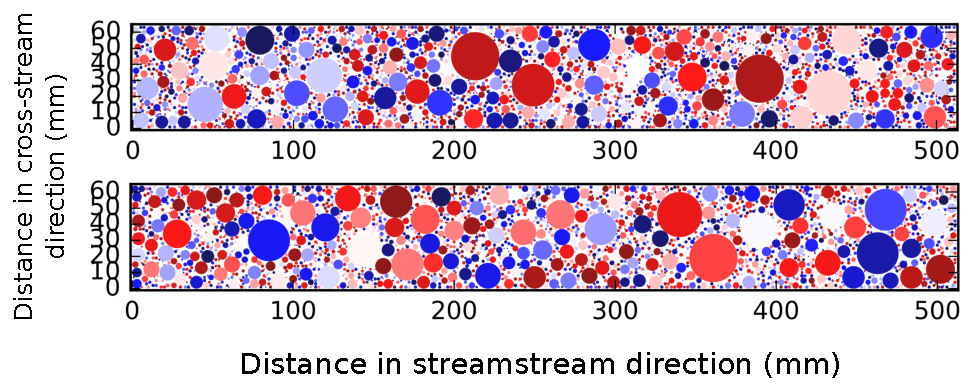
\includegraphics[width=0.90\textwidth]{Figures/Random_Beds.pdf}
		\caption{Graphic showing two random beds build with Part 1 of our code.}
	\label{Fig:RandomBed}
\end{figure}
The model consists of two different parts. Part 1 randomly builds a virtual streambed by placing spherical particles of diameter $D$ at open locations on the bed (Figures \ref{Fig:RandomBed} and \ref{Fig:3D}). The bed is rectangular in shape and should have a length $L$ longer than the range of particles travel distances. Locations on the bed are specified by model nodes, according to the grid resolution. The bed is filled with spheres until a specified 2D packing density is achieved. The present model can build a bed measuring 1028 mm x 128 mm of nonuniform particle size distribution ($\approx$ 5000 grains; Figures \ref{Fig:RandomBed} and \ref{Fig:3D}) and write the necessary files for 3D plotting in about 60 seconds. To simulate particle kinematics and a changing bed state, I think we need to specify the following particle quantities: (1) immigration rate, (2) emigration rate, (3) birth rate, (4) death rate, (5) particle velocity and (6) hop or travel distance. The key question to address for all of this seems to be whether or not we initialize and feed particles of uniform vs. non-uniform size distribution. Almost all the work to date used either a uniform or an almost uniform size distribution. So:
\begin{outline}
\1 \textbf{Question}: To start do we assume a uniform distribution of grain sizes of grain diameter $D$? If not, how do we express the entrainment rate as a function of grain size? The answer to this question will I think set the trajectory of how the remaining quantities are specified. Since all the work to date has been done with uniform grain sizes I think that is where we must start. I am not sure though.
\1 \textbf{Answer to Question}: To start we will assume either a uniform or a naorrowly graded distribution. At the moment, the model does well with a core grain size distribution for the approximate interval $[2,6]$ mm, with $D_g$ = 4.0 mm and $\sigma$ = 0.30. There is some small percentage of grains less than 2.0 mm diameter due to how the model revises grain radius if a placed grain is determined to overlap with an existing grain. We can of course shift the ditribution to a coarser range of sizes if desired, but with a similar magnitude of absolute size difference (i.e. 4.0 mm).
\end{outline}
David believes that hop distance $L_x$ is the key link between the Ancey and the Furbish group's work with respect to this modeling effort. We can likely neglect particle velocity $V_p$ and perhaps instead factor in the particle travel time $T_p$? Lets step though each quantity which will be represented within the model of particle motions. As above, I provide some initial questions about specifying each quantity as the discussion proceeds.
\begin{figure}[!ht]
	\centering
		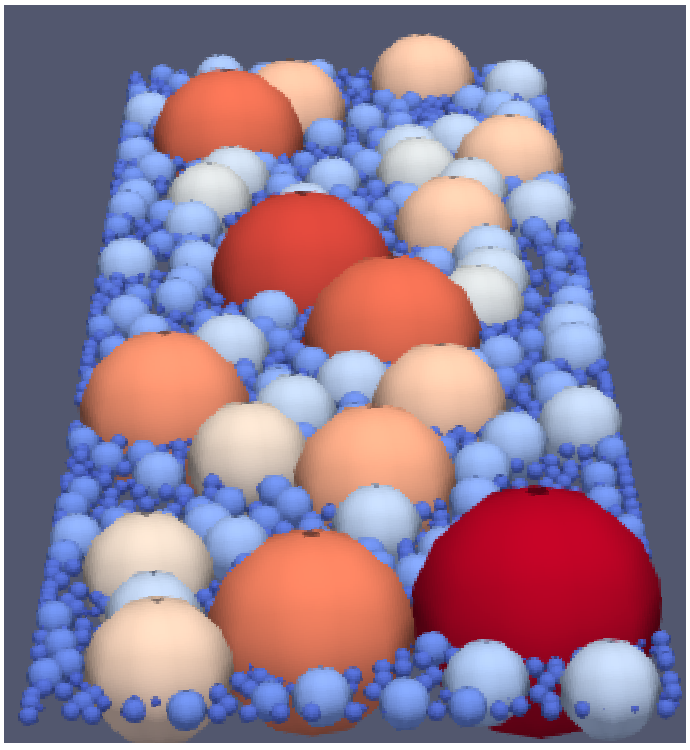
\includegraphics[width=0.5\textwidth]{Figures/Circles3D.pdf}
		\caption{Graphic showing a 3D represenation of a random bed built with Part 1 of our code. The plot is made in ParaView.}
	\label{Fig:3D}
\end{figure}
\begin{outline}[enumerate]
\1 \textbf{Model domain control volume--$V_c$} ($L^2$): The model domain streamwise length will be something like 2000 mm and the cross-stream length 100 mm. I think we will want $V$ to be of similar dimension to the experimental set-up of \citet{Ancey2010JGR}.
%
\1 \textbf{Immigration rate--$\nu_{in}$} (particles/t): For each small time increment $\Delta t$ it is possible that none, one or two+ particles up to some limit enters $V_c$. $\nu_{in}$ is specified by a sequence of random integers $0\rightarrow n$, for the approximate interval $[5,20]$ \citep{Ancey2010JGR}. Each particle will be introduced at the upstream boundary, and will have a randomly assigned grain diameter for the interval $[2,6]$ mm. Only integer values of diameter will be permitted for $\nu_{in}$ and will be set to zero for the first time step.
%
\1 \textbf{Emmigration rate--$\nu_{out}$} (particles/t): For each small time increment $\Delta t$ it is possible that none, one or two+ particles up to some limit leaves $V_c$. We may have to impose some hard limit to $\nu_{out}$ to avoid depletion of the virtual bed; alhtough this may be governed by the particle entrainment rate $\lambda_1$ and the hope distance $L_x$. $\nu_{out}$ will be determined based on $L_x$ applied to each entrianed grain. If $L_x$ is greater than the distance from the entrainment position to the downstream boundary than the specified particle emigrates. If $L_x$ is less than the distance from the entrainment position to the downstream boundary than the particle deposits, adding to $\sigma$. Deposition will not be permitted within the last $n$ rows within $V_c$. All of this means that $\nu_{out}$ will be internally determined based on the hop distance distribution and the number of particles $N$ in motion during any given time step.
%
\1 \textbf{Birth rate--$\lambda_1$} (particles/t): \citet{Ancey_et_al_2008} discuss that the number of particles entrained within $V_c$ by the flow is described by the rate parameter $\lambda_1$ [particles/t]. The inverse of $\lambda_1$ multiplied by number of entrainable particles is the waiting time $t^*$. If $\lambda_1$ is treated as a constant over all time, than the action of particle entrainment at one position in space is a Poisson point process; a relatively large collection of particles exhibiting this behavoir is considered a Poisson process, which is described by a Poisson distribution. Our goal is specify a birth or entrainment rate which reflects the conditions reported by \citet{Ancey_et_al_2008} and \citet{Ancey2010JGR}. Their work provides an approximated waiting time $t^*$ of $O(100-1000)$ seconds (time steps in our case) for low to moderate rates of particle entrainment. We calculate $\lambda_1$ as an exponentially distributed parameter at any small increment of time $\Delta t$:
\begin{equation}
	P_o(t)=exp(-A/E),
	\label{PoissonPoint_Simple}
\end{equation}
where $A$ is the actual number of entrained particles and $E$ is the expected number. \citet{Ancey2010JGR} reports that $E$ varies over the interval $[5,60]$. Here we use a value of 30 for $E$ and hold it steady for all simulation. The actual number of entrained particles varies randomly over a wider range of values than $E$. An exponential distribution for the actual number of entrained particles given $E=30$ implies a maximum value for $A$ of roughly 80 particles (i.e. $exp(-1)=0.37$. Therefore, we randomly sample $A$ for each time step over the interval $[5,80]$ for an exponential distribution given by equation \ref{PoissonPoint_Simple}. This gives us the total number of entrained particles over $V_c$ for each model time step.
%
\1 \textbf{Death rate--$\sigma$} (1/t): Depends on the total number of moving particles $N$ and can be calculated as the difference between the entrainment rate and the emmigration rate: $\sigma(N)=\lambda_1-\nu_{out}$. This thinking is associated with three implicite assumptions. First, all particles travel at the same velocity $V_x$. Second, particle hops and the hop distance $L_x$ are realized over some small, but single model time increment $\Delta t$. Last, the death rate is simply determined by whether a particle hop distance is large enough to remove the particle from $V_c$ via the downstream boundary. Therefore, if entrained partricles do not emmigrate, then the particles will come to rest within the vicinity of the end hop position (covered below).
%
\1 \textbf{Travel time--$T_p$} (t): \citep{Furbish2012a,Fathel2015,Furbish2017b} report that $T_p$ occurs over the interval $[0,1]s$ for their experiments. Why not start with this range of values? Note that the full range of travel times will occur within one simulation step or virtual time increment.
%
\1 \textbf{Hop distance--$L_x$} (L): \citet{Furbish2017b} specify that the hop distance has the form $L_x=aT_p^2+\epsilon$ where $a$ is a characteristic acceleration and $\epsilon$ is a stochastic deviation about the expected hop distance. \citet{Fathel2015} imply that $a\approx 1$, and so the expected hop distance can be modeled for $T_p$ over the interval $[0,1]s$ \citep{Furbish2012a,Fathel2015,Furbish2017b}. A different choice reported by \citet{Furbish2012a} provides that $L_x\sim T_p^{5/3}$. 
	\2 \textbf{Questions}: We can test both since each are a function of the particle travel time $T_p$?
%
\1 \textbf{Travel time deviation--$\epsilon$}: Could begin with an interval $[0,0.1]$?
%
\1 \textbf{Boundary conditions--BC}: We have several boundary conditions.
	\2 \textbf{Upstream boundary condition--$U_{BC}$}: Upstream boundary condition consists of the particle supply rate $\nu_{in}$. After the first simulation time step, $\nu_{in}=(\nu_{in})_{R,t}+(\nu_{out})_{t-1}$, where $R$ denotes the randomly chosen supply rate over the specified interval and $t-1$ is the previous model time step.
	\2 \textbf{Downstream boundary condition--$D_{BC}$}: Fix the downstream most 5 cm of particle numbers and elevations? (i.e. no deposition and no entrainment there?)
	\2 \textbf{Lateral boundary condition--$L_{BC}$}: No particles can leave the control volume via the lateral boundaries. I guess this implies all particles travel along fixed coordinate downstream paths. We could let particles move slightly laterally, but then it would be more difficult to identify internal controls on outcomes. Maintain our "keep it simple to start" perspective?
\1 \textbf{Grain placement with deposition}: Particles selected to move will have a randomly assigned hop distance $L_x$. If $L_x$ is shorter than the distance from the particle location $x$ to the last $x$ coordinate upstream from the downstream boundary condition, the particle will deposit. Grain stacking can occur in the event of deposition, but only to the extent of two particles high. We can choose deposition locations based on the closest minimum elevation to the point of deposition, within in some neighborhood radius. If there is no minimum elevation less than two particles high within the neigborhood than the particles will take one more jump. Avoiding vertical stacking greater than two particles high will avoid placement of particles in physically unrealistic ways? Something along these lines?
\end{outline}
\subsection{Calculation Procedure}
\begin{figure}[!ht]
	\centering
		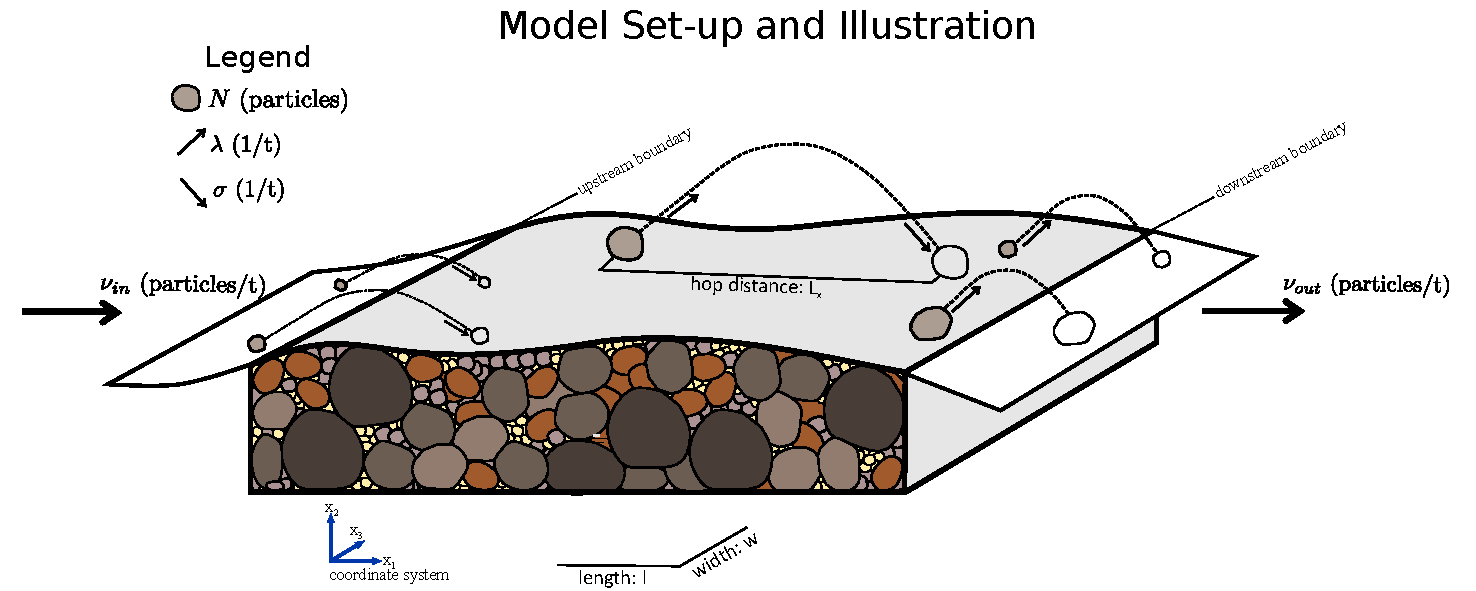
\includegraphics[width=1.1\textwidth]{Figures/Model_Setup.pdf}
		\caption{Illustration showing the model setup. See text for description of calculation procedures.}
	\label{Fig:Setup}
\end{figure}
Simulation of sediment transport for low to moderate transport rates will occur according to the following procedure:
\begin{outline}[enumerate]
\1 \textbf{For $t=1$ (time step)}
	\2 Specify $\nu_{in}=0$.
	%
	\2 Calculate $\lambda_1$ and specify $N_{total}=\lambda_1$
	%
	\2 Calculate $L_x$ for the number of entrained particles.
	%
	\2 Select grains for entrainment
	%
	\3 \textbf{Question}: How are particles selected for entrainment from among all available particles? Randomly across $V_c$ or is $V_c$ gridded and and then grids and particles are randomly selected?
	%
	\2 Calculate $\sigma$
	%
	\2 Calculate $\nu_{out}$
%
\1 \textbf{For $t\geq 1$}
	\2 $\nu_{in,t}=\nu_{out,t-1}$
	%
	\2 Calculate $\lambda_1$ and specify $N_{total}=\lambda_1+N_{total}$
	%
	\2 Repeat steps 1c-1f
\end{outline}
\begin{table}[h!]
	\caption{Model Build Parameter Values and Boundary Conditions}
	\centering
	\begin{tabular}{c c}
		\multicolumn{2}{c}{} \\[6pt]
		Parameter & Model Implementation \\
		\hline 
		\\[-0.5em]
		$GSD$ (L) & $[2,6]$; $D_g=4.0$ mm; $\sigma_g=0.30$ mm \\[6pt]
		$\nu_{in}$ (particles/t) & Random on the interval $[5,20]$ except for time step 1 \\[6pt]
		$\nu_{out}$ (1/t )& Internally controlled $\nu_{out}=[(\nu_{in}+\lambda_1)/N]-\sigma$ \\[6pt]
		$\lambda_1$ (1/t) & Exponentially distributed \\[6pt]
		$\sigma$ (1/t) & Entrained particles that do not hop out of the domain \\[6pt]
		$T_p$ (t) & $[0,1]$ \\[6pt]
		$L_x$ (L) & $L_x=aT_p^2+\epsilon$ \\[6pt]
		$\epsilon$ (t) & $[0,0.1]$ \\[6pt]
		\hline
		\\[-0.2em]
		\multicolumn{2}{l}{a. Downstream width change calculated for length scale $\varDelta x=$ 1.0 m} \\
		\label{Table1}
	\end{tabular}
\end{table}
\subsection{1D Deposition Procedure}
\begin{figure}[!ht]
	\centering
	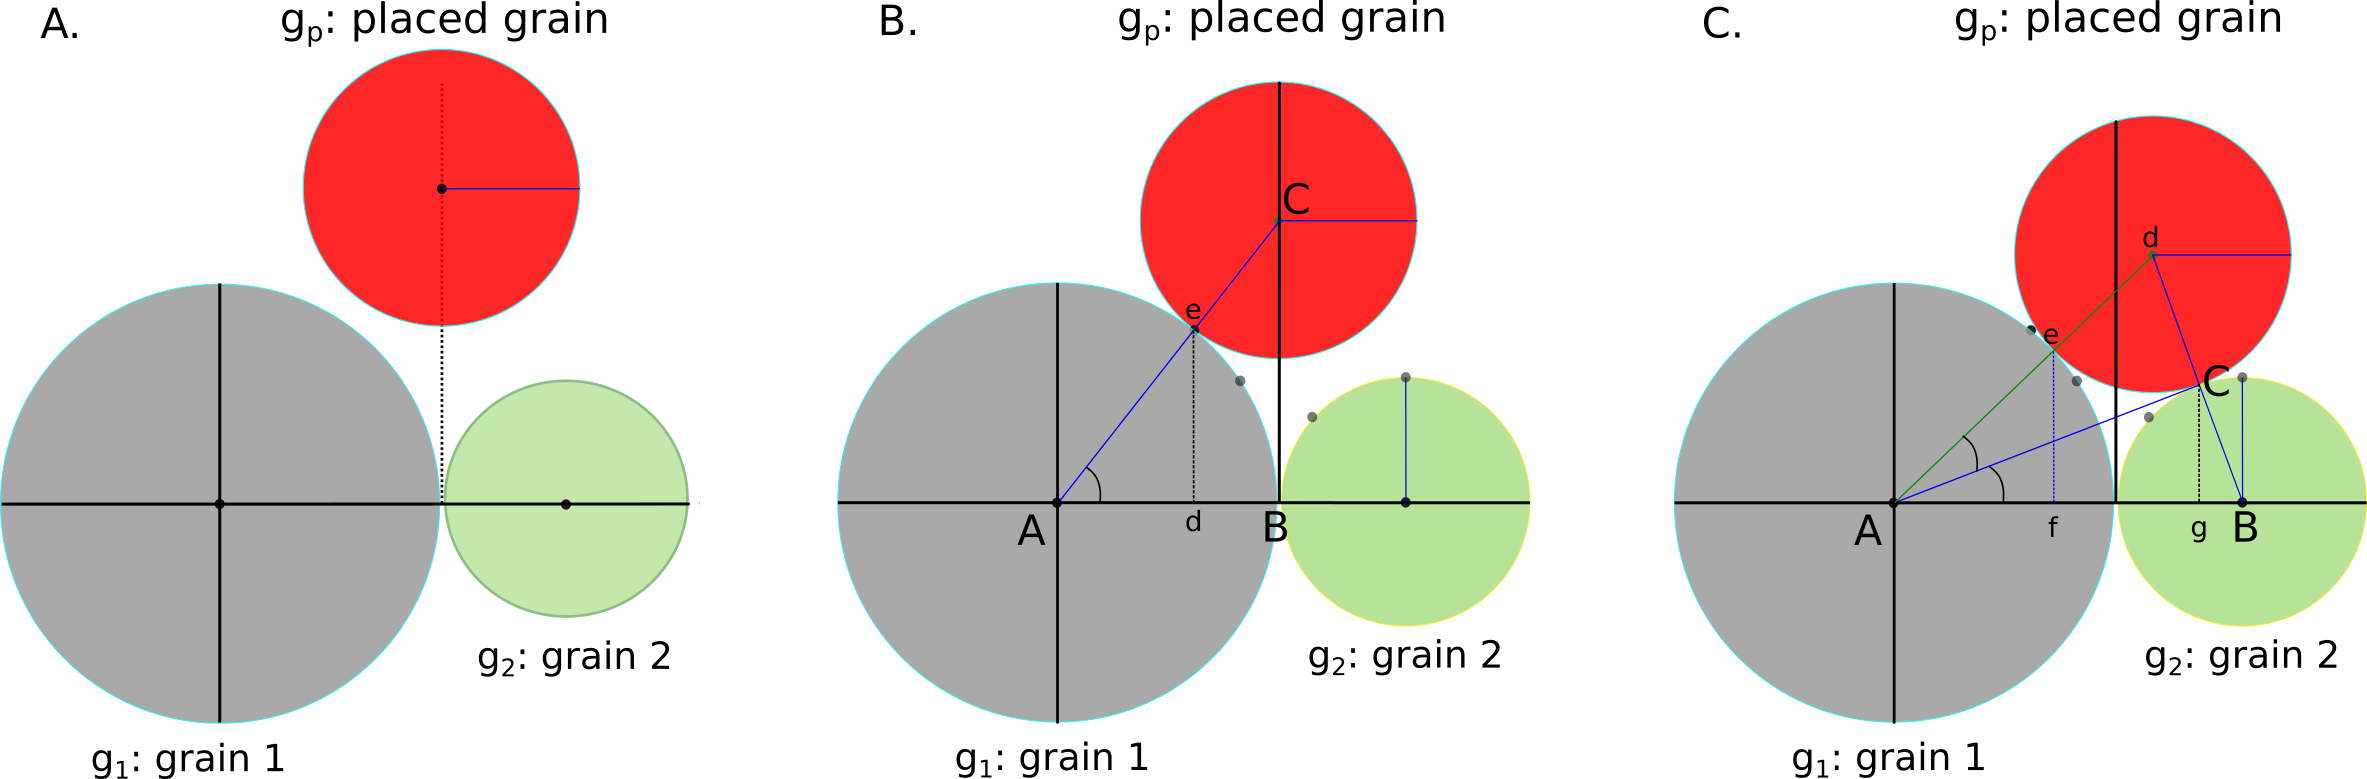
\includegraphics[width=0.90\textwidth]{Figures/1D_Deposition.png}
	\caption{Illustration showing how deposition position of placed grains is determined in the model. A: Basic set-up between placed grain and grains 1 and 2. B: Determination of first contact point as grain drops along vertex between two underlying grains. C: Determination of final two contact points between placed grain and grain 1, and placed grain and grain 2.}
	\label{Fig:Depo}
\end{figure}
\subsubsection{Initial Contact Point}
The placed grain drops along the projected vertex between grains 1 and 2. The initial contact between the placed grain and grain 1 is determined as (Figure \ref{Fig:Depo}B):
\begin{equation}
cos \measuredangle ABC = \frac{r_1}{r_1+r_p},
\label{Eqn 2}
\end{equation}
where $r_1$ is the radius of grain 1, and $r_1+r_p$ is the sum of radii of grain 1 and the placed grain. The angle $ABC$ is then simply $sin^{-1}(\frac{r_1}{r_1+r_p})$. The elevation of the initial contact point between grain 1 and the placed grain is then:
\begin{equation}
e_{elev} = 0 + (r_1sin \measuredangle ABC),
\label{Eqn 3}
\end{equation}
which with substitution using Equation \ref{Eqn 2} we have:
\begin{equation}
e_{elev} = 0 + \frac{r_1^2}{r_1+r_p}.
\label{Eqn 4}
\end{equation}
We assume an arbitrary elevation for the center of grain 1 of zero. The x-oriented position of $e$ is then:
\begin{equation}
g_{1,xc}+\overline{Ad} = g_{1,xc}+r_1cos \measuredangle ABC,
\label{Eqn 5}
\end{equation}
where $g_{1,xc}$ is the x-coordinate of the center of $g_1$. 
\subsubsection{Final Contact Points}
The final contact points between the placed grain and grain 2 is determined as (Figure \ref{Fig:Depo}C):
\begin{equation}
sin \measuredangle ABC = \frac{r_2}{r_1+r_2},
\label{Eqn 6}
\end{equation}
where $r_2$ is the radius of grain 2. The angle $ABC$  (Figure \ref{Fig:Depo}C) is then simply $sin^{-1}(\frac{r_2}{r_1+r_2})$. The x-oriented position of $C$ is then (projected down to point $g$):
\begin{equation}
g_{1,xc} + \overline{Ag} = g_{1,xc} + \frac{r_2}{sin \measuredangle ABC\cdot cos \measuredangle ABC},
\label{Eqn 7}
\end{equation}
and the elevation of point C is:
\begin{equation}
C_{elev} = 0 + \biggl(\frac{r_2\cdot tan \measuredangle ABC}{sin \measuredangle ABC\cdot cos \measuredangle ABC}\biggr),
\label{Eqn 8}
\end{equation}
The final contact point between the placed grain and grain 2 is determined:
\begin{equation}
tan \measuredangle CAd = \frac{r_p}{\frac{r_2}{sin \measuredangle ABC\cdot cos \measuredangle ABC}\cdot \frac{1}{cos \measuredangle ABC}},
\label{Eqn 9}
\end{equation}
with simplification provides:
\begin{equation}
tan \measuredangle CAd = \frac{r_p \cdot sin \measuredangle ABC\cdot cos^2 \measuredangle ABC}{r_2},
\label{Eqn 10}
\end{equation}
The angle $CAd$ is then simply $tan^{-1}(\frac{r_p \cdot sin \measuredangle ABC\cdot cos^2 \measuredangle ABC}{r_2})$. Last, the final contact points between grain 1 and the placed grain are given with the x-oriented position of $e$ (projected down to point $f$):
\begin{equation}
g_{1,xc}+\overline{Af} = g_{1,xc}+r_1cos \measuredangle Afe,
\label{Eqn 11}
\end{equation}
and the elevation of point e:
\begin{equation}
e_{elev}=0 + r_1sin \measuredangle Afe.
\label{Eqn 12}
\end{equation}
Note that the $\measuredangle Afe = \measuredangle CAd + \measuredangle ABC$ (Figure \ref{Fig:Depo}C).
\pagebreak
\section{Results}
\section{Discussion}
\section{Concluding remarks}
\pagebreak
List of Figures:
\begin{itemize}
\item{Fig1a: Schematic representation of 1-D, fixed width flume or channel showing a deterministic bed profile}
\item {Fig1b: Some sort of schematic image showing how turbulent flows can drive development of microstates of topography (bed grain size texture)?}
\item {Fig2: PR experimental data showing replicate profiles for 40, 60 and 80 lps runs. COuld also show 50m 70 and 90 lps runs}
\item {Fig3: P. Ashmore images - stacked in one figure showing variation of channel form of replicate experiments on stream table}
\item {Fig4: L. MacKenizie images - stacked in one figure showing variation of channel form of replicate experiments on stream table}
\item {Fig5: illustrations of model beds - 2D and 3D}
\item {Fig6: plots showing results}
\end{itemize}
List of Tables:
\begin{itemize}
\item {Tab1: Model parameter values, etc.}
\end{itemize}
\pagebreak
%%% End of body of article
%
% Notation
%
\begin{description}
\item[] List of Abbreviations and Symbols
\item{$A$} The flow area $L^2$
\item{$\overline{d}$} The average flow depth $L$
\item{$D_g$} Geometric mean grain size $L$
\item{$L_c$} Characteristic length scale $L$
\item{$\Delta\overline{\alpha}$} Downstream change in the average local width to flow depth ratio (-)
\item{$\varepsilon$} Solid fraction of the bed (-)
\item{$\eta$} Bed elevation $L$
\item{$\eta'$} Normalized average bed elevation (-)
\item{$\overline{\eta}'$} Normalized average bed elevation for the 12 subsampling locations (-)
\item{$\lambda$} Downstream spacing between sequential pools or riffles $L$
\item{$\varLambda$} Ratio of bed topography spreading to flow forcing time scales (-)
\item{$\nu$} The kinematic viscosity of water $L^2T$
\item{$\rho_w$} Density of water $ML^3$
\item{$\rho'$} $(\rho_w/\rho_s)-1$ (-)
\item{$\rho_s$} Density of sediment $ML^3$
\item{$\tau$} The average bed stress $ML^{-1}T^{-2}$
\item{$\tau*$} Dimensionless bed stress, referred to as "particle mobility" (-)
\item{$\hat{\tau}^*$} Normalized dimensionless bed stress, referred to as "particle mobility"(-) \item{$\tau_{c_{50}}^*$} The reference dimensionless critical bed stress for the 
\item{$D_{50}$} (-)
\item{$\tau_{ref}$} The reference average critical bed stress $ML^{-1}T^{-2}$
\item{$\tau_{ref}^*$} Equivalent to $\tau_{c_{50}}^*$ (-)
\item{$\phi$} Volume-averaged streambed porosity (-)
\item{$\chi$} Scaling factor (-)
\label{Ch3_tabnot}
\end{description}
%
\section{Acknowledgments}
SMC received funding from.....DJF received funding from..... Flume experiments were generously supported by an NSERC Discovery grant, and a Canada Foundation for Innovation grant to MH. Peter Ashmore graciously provided scans of his original PhD experiments at the University of Calgary. Lucy MacKenzie..... The authors report no financial conflicts of interest in completing this work or preparing this manuscript.\par 
%%  REFERENCE LIST AND TEXT CITATIONS
%    7. Bibliography
\bibliographystyle{plainnat}
\bibliography{SMCCurrentBib}
% TABLES
% FIGURES
\end{document}